\section{Ausgleichsrechnung / Interpolation}

Zur Auswertung Datenpunkte mit Streuung durch eine Funktion annähern.

\begin{description}
	\item[Interpolation] eine Funktion die exakt durch die Messpunkte geht.
		Geeignet falls:
		\begin{itemize}
			\item wenig Datenpunkte
			\item (fast) keine Messfehler
		\end{itemize}
	\item[Ausgleichsrechnung] eine Funktion die summiert die kleinste Abweichung
		von den Messpunkten hat. Zwischen den Messpunkten oftmals stabiler
		als Interpolation
		\begin{itemize}
			\item typischerweise viele Datenpunkte
			\item fehlerbehaftet
		\end{itemize}
\end{description}

\section{Interpolation}

\begin{itemize}
	\item Gegeben: \textcolor{red}{$n+1$} Wertepaare $(x_i, y_i), \, i = 0,...,n$
	      mit $x_i \ne x_j \, | \, i \ne j$
	\item Gesucht: stetige Funktion $g(x)$ mit $g(x_i) = y_i \, \forall i = 0,1,...,n$ \\
	      (was zwischen diesen Punkten für Resultate herauskommen kann stark variieren)
\end{itemize}


\subsection{Polynominterpolation}

Zu den $n+1$ Stützpunkten ist ein Polynom $P_n(x)
	= a_0 + a_1 x + a_2 x^2 + ... + a_n x^n$ vom Grad $n$ gesucht.

Weil das Polynom vom Grad $n$ ist lässt sich zusammen mit den Stützpunkten
ein lineares Gleichungsystem dazu aufstellen.

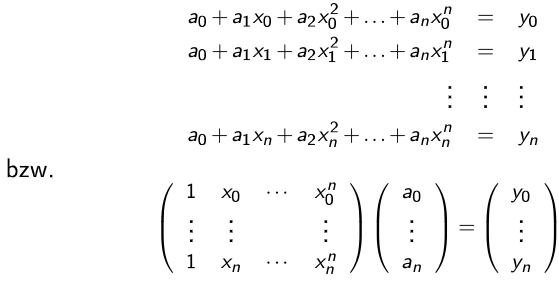
\includegraphics[scale=0.3]{interpol-poly-linearglgs}


\subsubsection{Lagrange Interpolationsformel}

Durch $n+1$ Stützpunkte mit verschiedenen Stützstellen gibt es genau EIN Polynom
$P_n(x)$ vom Grade $\le n$ welches alle Stützpunkte interpoliert.

Lagrangeform für $P_n(x)$:
$$P_n(x) = \sum_{i=0}^n l_i(x) y_i$$

Die Lagrangepolynome vom Grad $n$ ($l_i(x)$) sind definiert durch:
$$l_i(x) = \prod_{j=0, j \ne i}^n \frac{x - x_j}{x_i - x_j} \qquad \qquad i = 0,1,...,n$$

Beispiel:\\
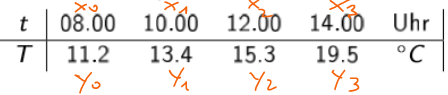
\includegraphics[scale=0.39]{interpol-poly-lagrange-bsp-data} \\
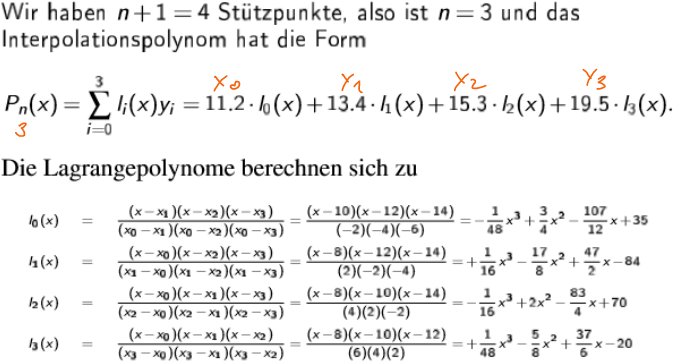
\includegraphics[scale=0.39]{interpol-poly-lagrange-bsp}


\subsubsection{Fehlerabschätzung}

Rein theoretisch weil man die tatsächliche Funktion $f$ kennen müsste.\\
Gegeben $y_i = f(x_i)$ und $f$ genügend oft stetig differenzierbar:

{
\Large
\begin{align*}
	|f(x) - P_n(x)| \quad \le \quad & \frac{|(x-x_0)(x-x_1)...(x-x_n)|}{(n+1)!}     \\
	                                & * \max_{x_0 \le \xi \le x_n} |f^{(n+1)}(\xi)|
\end{align*}
}



\subsection{Spline-Interpolation}

\subsubsection{Kontext (hoffentlich nicht Prüfungsrelevant)}

Die Annhäherung durch ein einziges Polynom ist zwischen den Messpunkten oft
hoch instabil. Als Alternative kann stattdessen stückweise interpoliert werden.

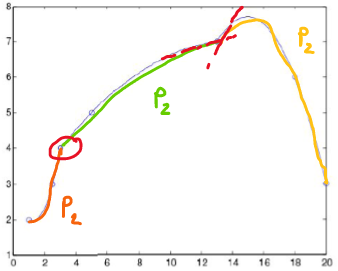
\includegraphics[scale=0.3]{interpol-split-poly-bsp}

\begin{itemize}
	\item hier stören die Knicke(Ableitung verschieden von beiden Seiten) an
	      den Übergängen
	\item die Spline-Interpolation versucht durch Polynome niederen Grades zu
	      interpolieren und damit Schwingungen unterdrücken $\rightarrow$ keine Knicke
	\item Polynome müssen dazu an den Messpunkten nicht nur selben Funktionswert
	      sondern auch selbe Ableitung haben (1. und 2. Ableitung).
\end{itemize}

Man kann so für jedes Interval $[x_i, x_{i+1}], \quad i = 0,1,2,...,n-1$ genau
ein Polynom $s_i$ ansetzen ($i$ Bezeichnet die Nummer des Intervalls).

Dieses Polynom muss folgende Bedingungen erfüllen:
{\large
\begin{description}[itemsep=1mm]
	\item[Interpolation] $s_i(x_i) \, = \, y_i \quad,
			\quad s_{i+1}(x_{i+1}) \, = \, y_{i+1}$
	\item[stetiger Übergang] $s_i(x_{i+1}) \, = \, s_{i+1}(x_{i+1}) \quad,
			\quad s_{i+1}(x_{i+2}) \, = \, s_{i+2}(x_{i+2})$
	\item[keine Knicke] $s'_i(x_{i+1}) = s'_{i+1}(x_{i+1}) \quad,
			\quad s'_{i+1}(x_{i+2}) = s'_{i+2}(x_{i+2})$
	\item[gleiche Krümmung] $s''_i(x_{i+1}) \, = \, s''_{i+1}(x_{i+1}) \quad,
			\quad s''_{i+1}(x_{i+2}) \, = \, s''_{i+2}(x_{i+2})$
	\item[Zusatzbedingungen] Damit es genug Gleichungen für ein reguläres System
		sind müssen noch Zusatzbediungen gesetzt werden, diese unterscheiden sich
		je nach Art des gewählten Splines
\end{description}
}

Beispiel (6.5 in Folien):\\
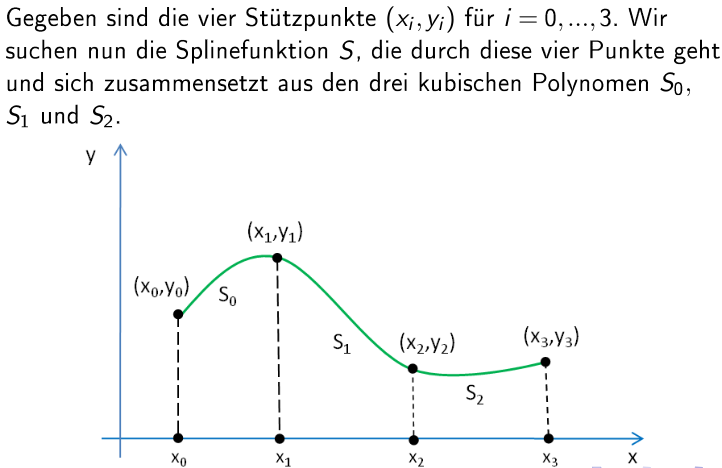
\includegraphics[scale=0.26]{interpol-spline-bsp-ausgang}\\
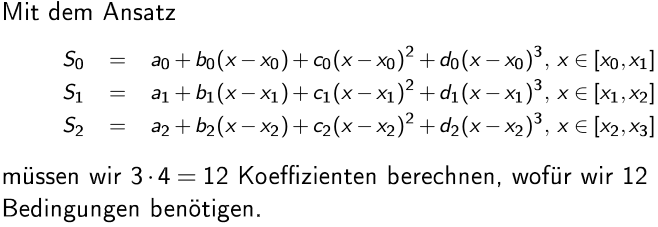
\includegraphics[scale=0.28]{interpol-spline-bsp-ansatz}\\
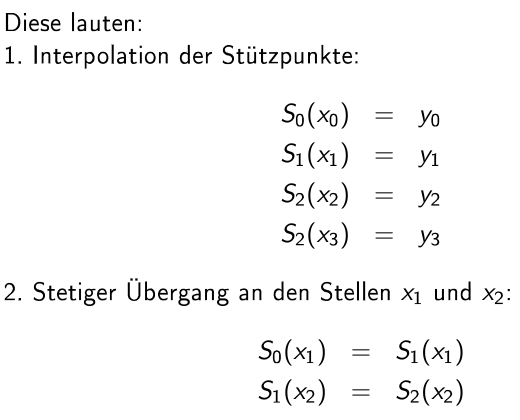
\includegraphics[scale=0.26]{interpol-spline-bsp-bedingungen1}\\
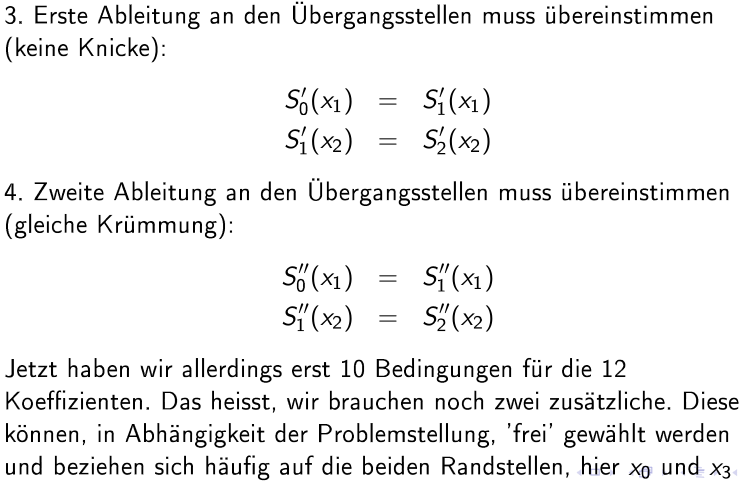
\includegraphics[scale=0.26]{interpol-spline-bsp-bedingungen2}\\
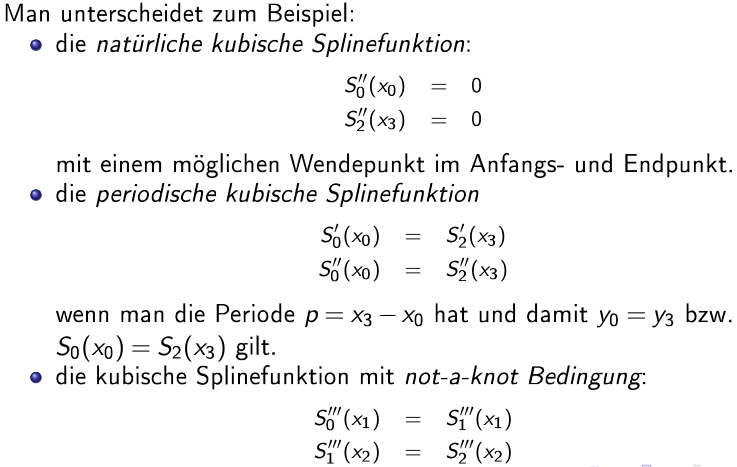
\includegraphics[scale=0.3]{interpol-spline-bsp-zusatzbedingungen}\\




\subsubsection{natürliche kubische Splinefunktion}
%TODO code
Gegeben $n+1$ Stützpunkte $(x_i, y_i)$ mit monoton aufsteigenden
Stützstellen $x_0 < x_1 < ... < x_n \quad | \quad \mathrm{und}\; n \ge 2$

Gesucht natürliche kubische Splinefunktion $S(x)$,
in jedem Intervall $[x_i, x_{i+1}]\, ,\,i=0,1,...,n-1$ definiert durch das Polynom

	{\large
		$$S_i(x) = a_i + b_i(x-x_i) + c_i(x-x_i)^2 + d_i(x-x_i)^3$$
	}

Als Gleichungsystem $Ac = z$ (nur für $c_i$, entspricht 4. aus Algorithmus)

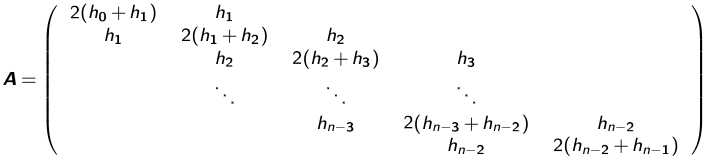
\includegraphics[scale=0.35]{interpol-spline-algo-A}\\
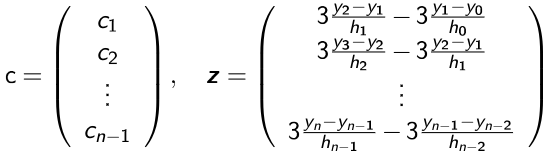
\includegraphics[scale=0.3]{interpol-spline-algo-cz}


\begin{minipage}{0.4\linewidth}
	Beispiel als Tabelle für manuelle Berechnung:
\end{minipage}
\hfill
\begin{minipage}{0.5\linewidth}
	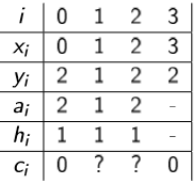
\includegraphics[scale=0.3]{interpol-spline-bsp-tabelle}
\end{minipage}

\textcolor{blue}{\Large Kompletter Algorithmus}

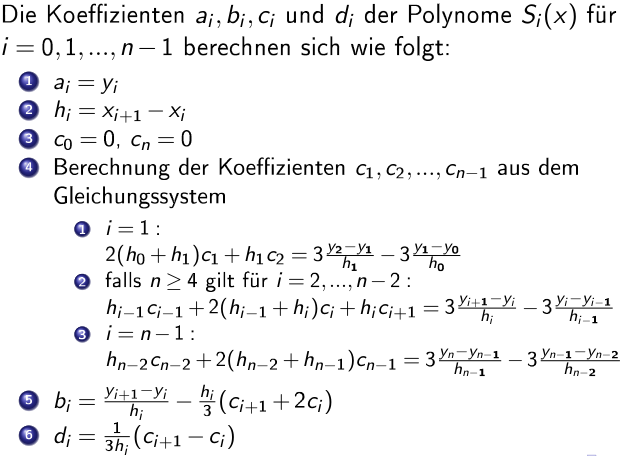
\includegraphics[scale=0.4]{interpol-spline-natkubisch-algo}




\section{Ausgleichsrechnung}
Unterschied zur Interpolation: Funktion soll nicht exakt durch alle Messpunkte
gehen sondern möglichst gut approximieren $\rightarrow$ stabileres Verhalten
abseits der Messpunkte.\\
Besonders sinnvoll bei vielen Daten (meist zusätzlich fehlerbehaftet)

\subsubsection{Ausgleichsproblem}

Gegeben Wertepaare $(x_i, y_i) \; i = 1,...,n$ mit $x_i \ne x_j \; | \; i \ne j$

Gesucht stetige Funktion $f: \R \to \R$ die bestmöglich Annähert. Heisst
$f(x_i) \approx y_i$


\subsubsection{Ansatzfunktionen/Ausgleichsfunktion/Fehlerfunktional/
	kleinste Fehlerquadrate}

Gegeben:
\begin{itemize}
	\item Menge $F$ von stetigen \textcolor{blue}{Ansatzfunktionen} $f$
	\item $n$ Wertepaare $(x_i,y_i)$
\end{itemize}

Eine Funktion $f \in F$ heisst \textcolor{blue}{Ausgleichsfunktion} von $F$ zu
den Wertepaaren, falls das \textcolor{blue}{Fehlerfunktional} $E$ minimal wird.\\
Das $f$ mit dem minimum nennt man optimal im Sinne der \textcolor{blue}{kleinsten
Fehlerquadrate}


{\large
$$E(f) = ||y-f(x)||^2_2 = \sum^n_{i=1}(y_i - f(x_i))^2$$
}




\subsection{lineare Ausgleichsrechnung}

Gesuchte Funktion $f$ ist Linearkombination vom $m$ Basisfunktionen $f_i,
	\; i = 1,2,...,m \; | \; m \le n$ und den gesuchten Parametern $\lambda_i$

Wenn $m \le n$ ist das Gleichungsystem überbestimmt und es existiert keine Lösung
$E(f) = 0$, ist $m = n$ gibt es diese Lösung jedoch und wir sind wieder beim
Spezialfall der Interpolation

$$f(x) = \lambda_1 f_1(x) + ... + \lambda_m f_m(x)$$

\subsubsection{Lineares Ausgleichsproblem}
%TODO code
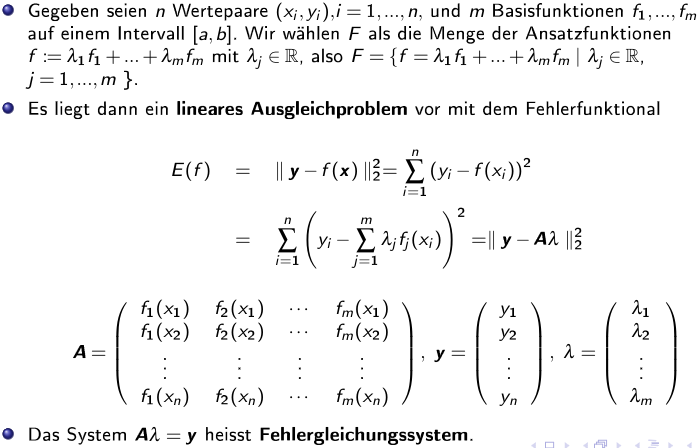
\includegraphics[scale=0.38]{ausgleich-lin-problem-def}


\subsubsection{Normalengleichung}

Um das Fehlerfunktional zu minimieren müssen alle partiellen Ableitungen von
$E(f)$ verschwinden, also {\Large $\frac{\partial E(f)}{\partial \lambda_j} = 0$}


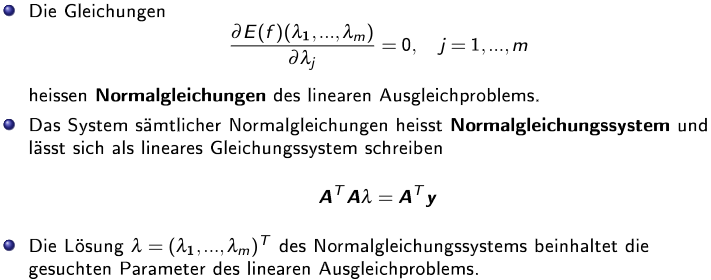
\includegraphics[scale=0.38]{ausgleich-lin-normalenglg}

\textcolor{red}{Weil $A^T A$ aber oft schlecht konditioniert ist wird $A$ mittels
	QR-Verfahren zerlegt
}
{\Large
	$$A^T A \lambda = A^T y \rightarrow A = QR \rightarrow R \lambda = Q^T y$$
}





\subsection{nichtlineare Ausgleichsrechnung}

Parameter $\lambda$ treten verwoben in der Funktion $f$ auf

$$f = f(\lambda_1, ..., \lambda_m, x)$$

\subsubsection{nichtlineare Ausgleichsprobleme}

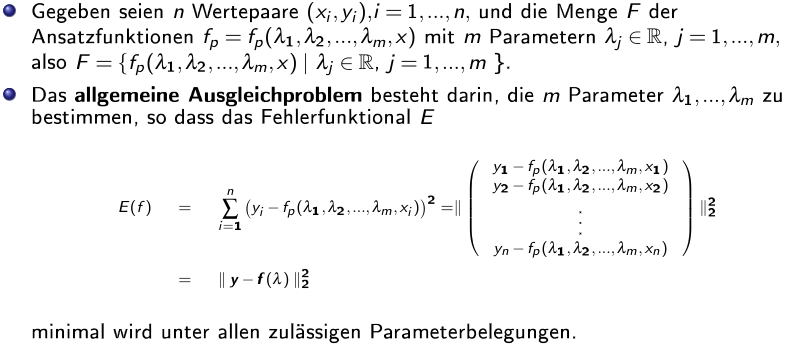
\includegraphics[scale=0.34]{ausgleich-nichtlin-allg-ausgleichprob}

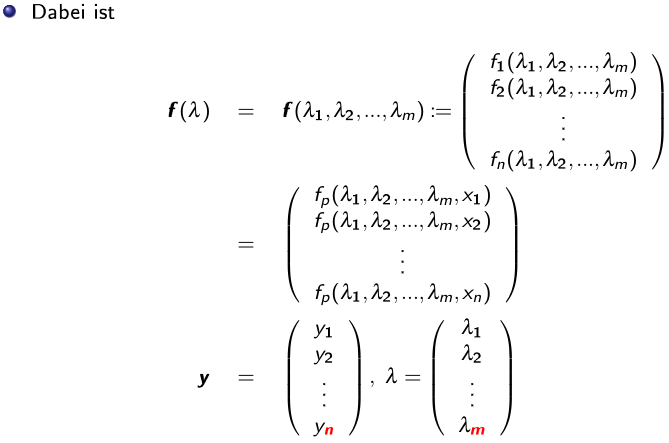
\includegraphics[scale=0.31]{ausgleich-nichtlin-allg-ausgleichprob2}



\subsubsection{Quadratmittelproblem}

Gegeben Funktion $\v g: \R^m \to \R^n$ und zugehöriges Fehlerfunktional
$E: \R^m \to \R \; = || \v g(x) ||_2^2$ \\
Das Problem $\v x \in \R^m$ zu finden für den $E(x)$ minimal wird heisst
Quadratmittelproblem.

\textcolor{cyan}{nichtlineare Ausgleichsprobleme sind Quadratmittelprobleme
	mit $\v g(x) = \v g(\lambda)$.}
Als Fehlerfunktional dient die differenz zwischen dem tatsächlichen Wert und dem
Wert der Funktion $\v f$.

	{\large
		$$\v g(\v \lambda) = \v y - \v f(\v \lambda), \v y \in \R^n, \v \lambda \in \R^m$$
	}



\subsubsection{Gauss Newton-Verfahren}
% TODO code

\begin{itemize}
	\item Kombination aus linearer Ausgleichsrechnung und Newton-Verfahren
	\item In $||\v g(\lambda) ||_2^2$ wird $\v g(\lambda)$ ersetzt durch folgende
	      Linearkombination
		      {\large
			      $$\v g(\lambda) \approx \v  g(\lambda^{(0)}) + D\v g(\lambda^{(0)}) * (\lambda
				      - \lambda^{(0)})$$
		      }
	\item $Dg(..)$ entspricht hierbei der Jacobi-Matrix von $\v g$
    \item Durch folgende Substitutionen haben wir die Form einer linearen Ausgleichsrechnung
        $E(\lambda) = ||y - A \delta||_2^2$
        \begin{description}
            \item[$y$] $= \v g(\lambda^{(0)})$
            \item[$A$] $= -D\v g(\lambda^{(0)})$
            \item[$\delta$] $= \lambda - \lambda^{(0)}$
        \end{description}
\end{itemize}



% TODO replace with custom copy
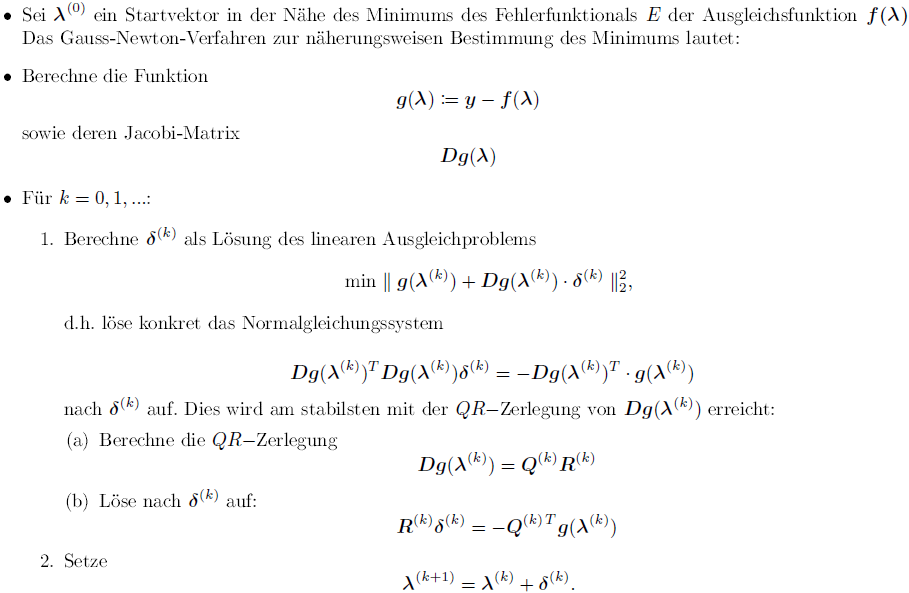
\includegraphics[width=\linewidth]{ausgleich-nichtlin-gauss-newton-algo}




